%%%%%%%%%%%%%%%%%%%%%%%%%%%%%%%%%%%%%%%%%%%%%%%%%%%%%%%%%%%%%%%%%%%%%%%%%%%%%%
%%
%%
%%  
%%  奈良工業高等専門学校 情報工学科
%%
%%  第 4 学年 情報工学実験 III
%%
%%        「コンピュータネットワークに関する実験」実験報告書
%%
%%                作成日 平成 28 年  7月 8 日 金(PDFpLaTeX 版)
%%                提出日 平成 28 年  67月 8 日 金(PDFpLaTeX 版)
%%
%%            池内隆一郎 (an94_49@yahoo.co.jp)
%%
%%
%%%%%%%%%%%%%%%%%%%%%%%%%%%%%%%%%%%%%%%%%%%%%%%%%%%%%%%%%%%%%%%%%%%%%%%%%%%%%%

\documentclass[12pt]{jreport}

\setlength{\topmargin}{-12.5truemm}

\setlength{\textheight}{\paperheight}   % 紙面縦幅を本文領域にする(BOTTOM=-TOP)
\setlength{\topmargin}{-5.4truemm}      % 上の余白を20mm(=1inch-5.4mm)に
\addtolength{\topmargin}{-\headheight}  % 
\addtolength{\topmargin}{-\headsep}     % ヘッダの分だけ本文領域を移動させる
\addtolength{\textheight}{-50truemm}    % 下の余白は30mm(BOTTOM=-TOPだから+TOP+30mm)
\setlength{\textwidth}{\paperwidth}     % 紙面横幅を本文領域にする(RIGHT=-LEFT)
\setlength{\oddsidemargin}{-5.4truemm}  % 左の余白を20mm(=1inch-5.4mm)に
\setlength{\evensidemargin}{-5.4truemm} % 
\addtolength{\textwidth}{-40truemm}     % 右の余白も20mm(RIGHT=-LEFT)

% \usepackage[dviout]{graphicx}
\usepackage{comment}    % comment 環境を使うためのスタイルファイル

\usepackage{listings}

%
%    ↓丸みのある四角や影付きの四角などを使うためのスタイルファイル
%
\usepackage{fancybox}    % shadowbox, ovalbox 環境を使うためのスタイルファイル
\usepackage{ascmac}    % screen 環境を使うためのスタイルファイル
\usepackage{framed}    % framed 環境を使うためのスタイルファイル

%
%    ↓PostScript 形式 や EPS 形式の図を張り付けるためのスタイルファイル
%
\usepackage{float}    % 図や表を記述した位置に置くためのスタイルファイル
\usepackage[dvipdfmx]{graphicx}    % 回転などもできるスタイルファイル

%
%    箇条書きに関するスタイルファイル
%
\usepackage{enumitem}    % 拡張 enumerate 環境を使うためのスタイルファイル

\makeatother
\title{コンピュータネットワークに関する実験 \vspace{5cm}}
\author{\hspace{10cm} 4 年 情報工学科 2番 \\\\\hspace{9cm} 提出者: 1班 池内 隆一郎}
\date{\vspace{1cm}\hspace{-10cm}提出締め切り: 平成28年7月8日(金)\\ \\ \hspace{-120mm} 提出日: 平成28年 7月8日(金)\\\hspace{-143mm} \\ \hspace{-143mm}共同実験者
\begin{description}
\setlength{\parskip}{0.1mm}
\item1番 安西崇 \item3番 石田豊美 \item4番 荻野春樹
\item5番 茅野哲也 \item6番 黒田滉平 \item7番 鴻上遼河
\end{description}}

\begin{document}
    
    \maketitle
    \newpage

    \chapter*{第1章 アブストラクト}

    \chapter*{第2章 実験結果}
        \section*{2.1 実験1 Unixの基本コマンドの習得}
            \subsection*{2.1.1 課題1-1}
                lsコマンドの引数に正規表現を指定して、各自に与えられたログインユーザーのホームディレクトリにある環境設定ファイルのみを表示する。図1に正規表現を使用した環境設定ファイルのコマンドと出力を示す。
                \begin{figure}[H]
                    \begin{center}
                        \begin{screen}
                            \begin{verbatim}
mint02<~>[1]% pwd
/home/staff/mint02
mint02<~>[2]% ls -ldg .[a-zA-Z]*
total 50
-rw-------  1 mint02  mint     0  4月 11 14:38 .Xauthority(*)
-rw-r--r--  1 mint02  mint  1482  3月 25  2011 .Xdefaults
-rw-r--r--  1 mint02  mint  2463  3月 25  2011 .Xresources
drwx------  2 mint02  mint   512  4月 11 17:33 .autosave
-rw-r--r--  1 mint02  mint   165  3月 25  2011 .bashrc
-rw-r--r--  1 mint02  mint  4528  3月 25  2011 .canna
-rw-r--r--  1 mint02  mint  7704  3月 25  2011 .canna-default
-rw-r--r--  1 mint02  mint   164  3月 25  2011 .cshrc
-rw-r--r--  1 mint02  mint   276  3月 25  2011 .emacs
-rw-r--r--  1 mint02  mint    40  3月 25  2011 .emacs-mule
-rw-r--r--  1 mint02  mint   222  3月 25  2011 .emacs-xemacs
-rw-r--r--  1 mint02  mint   505  3月 25  2011 .emacs.mew
-rw-r--r--  1 mint02  mint    36  3月 25  2011 .fvwmrc
-rw-r--r--  1 mint02  mint    36  3月 25  2011 .fvwmrc
-rw-------  1 mint02  mint  1159  4月 11 17:42 .history
-rw-r--r--  1 mint02  mint   164  3月 25  2011 .login
-rw-r--r--  1 mint02  mint     0  3月 25  2011 .nosxsession
-rw-r--r--  1 mint02  mint  4047  3月  8  2014 .vimrc
drwxr-xr-x  2 mint02  mint   512  3月 25  2011 .xemacs
-rw-r--r--  1 mint02  mint   340  3月 25  2011 .xmodmap
-rwxr-xr-x  1 mint02  mint  1119  3月 25  2011 .xsession
-rw-------  1 mint02  mint   830  4月 11 17:45 .xsession-errors
-rw-r--r--  1 mint02  mint   165  3月 25  2011 .zshenv
-rw-r--r--  1 mint02  mint   162  3月 25  2011 .zshrc
                            \end{verbatim}
                        \end{screen}
                        \caption{正規表現を使用した環境設定ファイルの表示}
                        \label{1}
                    \end{center}
                \end{figure}
            lsコマンドはディレクトリを表示させるコマンドである。オプションは-lで、ファイル名だけでなくタイムスタンプやパーミッション、オーナー情報も表示させる。-dでディレクトリの中身ではなく、そのディレクトリ自体を表示させることができる。-gは-lのファイルオーナーのグループ名を表示しないというオプションだが、-lをつけている場合は付けても付けなくても同じである。正規表現は、"[]"を用いて"[]"内の文字一文字に一致しているかどうか判定、"*"でそれを繰り返すことにより"."から始まって小文字、大文字のアルファベットが続くファイルのみを表示させる。

            図2に簡単化した環境設定ファイルのコマンドと出力を示す。(FreeBSD10.3) また、図2のコマンドで環境設定ファイルとカレントディレクトリと親ディレクトリを表示させる。図1のコマンドは長いので、通常普通に使いたいだけの場合は図2のコマンドを使うほうが良い。
                \begin{figure}[H]
                    \begin{center}
                        \begin{screen}
                            \begin{verbatim}
mint02:~ % ls -ldA .*
drwxr-xr-x  2 i9270  i9270   512 Jul  5 05:36 .
drwxr-xr-x  3 root   wheel   512 Jul  5 05:25 ..
-rw-r--r--  1 i9270  i9270  1066 Jul  5 05:25 .cshrc
-rw-------  1 i9270  i9270   165 Jul  5 05:40 .history
-rw-r--r--  1 i9270  i9270   252 Jul  5 05:25 .login
-rw-r--r--  1 i9270  i9270   163 Jul  5 05:25 .login_conf
-rw-------  1 i9270  i9270   379 Jul  5 05:25 .mail_aliases
-rw-r--r--  1 i9270  i9270   336 Jul  5 05:25 .mailrc
-rw-r--r--  1 i9270  i9270   817 Jul  5 05:25 .profile
-rw-------  1 i9270  i9270   281 Jul  5 05:25 .rhosts
-rw-r--r--  1 i9270  i9270   978 Jul  5 05:25 .shrc
                            \end{verbatim}
                        \end{screen}
                        \caption{簡単化した環境設定ファイルの表示}
                        \label{2}
                    \end{center}
                \end{figure}

            \subsection*{2.1.2 課題1-2}
                各自与えられたログインユーザーのホームディレクトリにnewmemberディレクトリを作成する。図3にnewmemberディレクトリを作成するコマンドを示す。
                \begin{figure}[H]
                    \begin{center}
                        \begin{screen}
                            \begin{verbatim}
mint02<~>[1]% mkdir newmember
mint02<~>[2]%
                            \end{verbatim}
                        \end{screen}
                        \caption{ディレクトリ作成コマンド}
                        \label{3}
                    \end{center}
                \end{figure}
                図3のmkdirコマンドによりディレクトリを作成することができる。また、属性は755でオーナーはmkdirを実行したユーザーになる。

            \subsection*{2.1.3 課題1-3}
                課題1-2で作成したnewmemberディレクトリの許可属性を以下に示すように、所有者のみに、「Read属性」、「Write属性」、「eXecute属性」を与え、グループやその他のユーザーからすべての属性を削除する。
                \begin{figure}[H]
                    \begin{center}
                        \begin{screen}
                            \begin{verbatim}
mint02<~>[1]% chmod 700 newmember
mint02<~>[2]
                            \end{verbatim}
                        \end{screen}
                        \caption{属性変更コマンド}
                        \label{4}
                    \end{center}
                \end{figure}
                図4のchmodコマンドで属性を変更する。700は左から、所有者権限、グループ権限、その他ユーザー権限を表す。また、7は「Read属性」、「Write属性」、「eXecute属性」のすべてを与えるという意味であり、0はすべてを与えないという意味である。他にも、u+rwxなど使い権限変更をできるが、手間であるため、こちらの数字を用いるのが一般的である。

            \subsection*{2.1.4 課題1-4}
                ログインユーザ名nishinoのホームディレクトリの中にある2016-4I.pwdファイルをnewmemberディレクトリにコピーする。図5にファイルをコピーするコマンドを示す。

                \begin{figure}[H]
                    \begin{center}
                        \begin{screen}
                            \begin{verbatim}
mint02<~>[1]% pwd
/home/stuff/mint02
mint02<~>[2]% cp ../nishino/2016-4I.pwd newmember/
                            \end{verbatim}
                        \end{screen}
                        \caption{ファイルをコピーするコマンド}
                        \label{5}
                    \end{center}
                \end{figure}
                ファイルやディレクトリをコピーするには、図5に示すようにcpコマンドを用いる。第1引数でコピーするファイルやディレクトリを指定し、第2引数でコピー先を指定する。図5のコマンドの場合、ファイル(../nishino/2016-4I.pwd)をディレクトリ(newmember/)に移動する。また、ディレクトリをコピーする場合は-rオプションを付けることによりディレクトリ内のファイルやディレクトリを再帰的にコピーすることができる。

            \subsection*{2.1.5 課題1-5}
                課題1-2で作成したnewmemberディレクトリに移動(カレントディレクトリの変更)。図6にディレクトリを変更するコマンドを示す。
                \begin{figure}[H]
                    \begin{center}
                        \begin{screen}
                            \begin{verbatim}
mint02<~>[1]% pwd
/home/stuff/mint02
mint02<~>[2]% cd newmember/
mint02<~>[3]% pwd
/home/stuff/mint02/newmember
                            \end{verbatim}
                        \end{screen}
                        \caption{ディレクトリを変更するコマンド}
                        \label{6}
                    \end{center}
                \end{figure}
                ディレクトリの変更には図6のようにcdコマンドを使用する。引数にディレクトリを指定することにより、指定したディレクトリに移動することができることが確認できる。

            \subsection*{2.1.6 課題1-6}
                grepコマンドを使用して、2016-4I.pwdファイルから自分を含む実験メンバーを抽出し、その内容をユーザーごとに、その内容をユーザー毎に「innnn.pwd」ファイル(nnnnは、各ユーザの4桁の学籍番号)に保存する。図7にファイルから抜き出し別のファイルに保存するコマンドを示す。
                \begin{figure}[H]
                    \begin{center}
                        \begin{screen}
                            \begin{verbatim}
mint02<~>[1]% cat 2016-4I.pwd | grep i9269 > i9269.pwd
mint02<~>[2]% cat 2016-4I.pwd | grep i9270 > i9270.pwd
mint02<~>[3]% cat 2016-4I.pwd | grep i9271 > i9271.pwd
mint02<~>[4]% cat 2016-4I.pwd | grep i9274 > i9274.pwd
mint02<~>[5]% cat 2016-4I.pwd | grep i9275 > i9275.pwd
mint02<~>[6]% cat 2016-4I.pwd | grep i9276 > i9276.pwd
mint02<~>[7]% cat 2016-4I.pwd | grep i9277 > i9277.pwd
                            \end{verbatim}
                        \end{screen}
                        \caption{ファイルから抜き出し別のファイルに保存するコマンド}
                        \label{7}
                    \end{center}
                \end{figure}
                catコマンドを用いることにより、標準出力(コンソール)にファイルを出力することができる。引数はファイル名である。"\textbar"はパイプ機能である。左のコマンドの出力を右に受け渡すことにより、catコマンドの出力をgrepコマンドを用いることによって検索を行い一致した行だけを出力することができる。''\verb|>|''は指定することができる。今回の場合引数に''\verb|>|''の後にファイル名がきているのでそのファイルに出力する。また、''\verb|>|\verb|>|''を使えば、ファイルに追記することも可能である。ちなみに''\verb|<|''を使って標準入力を変えることも可能である。
                図7のコマンドでは、''cat 2016-4I.pwd''で2016-4I.pwdの中身をgrepに渡し、それをgrepがinnnnという文字列で検索を行い、引っかかった行をinnn.pwdファイルに出力している。

            \subsection*{2.1.7 課題1-7}
                自分を含む各実験メンバーが抽出された「innnn.pwd」ファイルの内容を結合し、group\_1.pwdファイルに保存する。図8にファイルを結合するコマンドを示す。
                \begin{figure}[H]
                    \begin{center}
                        \begin{screen}
                            \begin{verbatim}
mint02<~>[1]% cat i9269.pwd >> group_1.pwd
mint02<~>[2]% cat i9270.pwd >> group_1.pwd
mint02<~>[3]% cat i9271.pwd >> group_1.pwd
mint02<~>[4]% cat i9274.pwd >> group_1.pwd
mint02<~>[5]% cat i9275.pwd >> group_1.pwd
mint02<~>[6]% cat i9276.pwd >> group_1.pwd
mint02<~>[7]% cat i9277.pwd >> group_1.pwd
                            \end{verbatim}
                        \end{screen}
                        \caption{ファイル結合のコマンド}
                        \label{8}
                    \end{center}
                \end{figure}
                ''\verb|>|\verb|>|''を用いることにファイルに追記することができる。図8では、innnn.pwdファイルの中身をgroup\_1.pwdに追記していくことによって、group\_1.pwdへファイルを結合していく。

            \subsection*{2.1.8 課題1-8}
                課題1-7で作成したgroup\_g.pwdファイルの名前をmembers\_master.pwdに変更する。
                \begin{figure}[H]
                    \begin{center}
                        \begin{screen}
                            \begin{verbatim}
mint02<~>[1]% ls
2016-4I.pwd
mint02<~>[2]% mv group_1.pwd members_master.pwd
mint02<~>[3]% ls
members_master.pwd
                            \end{verbatim}
                        \end{screen}
                        \caption{ファイル名変更コマンド}
                        \label{9}
                    \end{center}
                \end{figure}
                名前の変更にはmvコマンドを用いる第1引数に元のファイル名を指定し、第2引数に新しいファイルの名前を指定する。図9ではgroup\_1.pwdという名前のファイルをmembers\_master.pwdという名前に変更していることを確認できる。

            \subsection*{2.1.9 課題1-9}
                members\_master.pwdファイルの許可属性を所有者のみに「Read属性」、「Write属性」を与え、グループやその他のユーザーからすべての属性を削除する。図10に許可属性変更のコマンドを示す。
                \begin{figure}[H]
                    \begin{center}
                        \begin{screen}
                            \begin{verbatim}
mint02<~>[2]% chmod 600 members_master.pwd
                            \end{verbatim}
                        \end{screen}
                        \caption{許可属性変更コマンド}
                        \label{10}
                    \end{center}
                \end{figure}
                2.1.3と同じくchmodを使い許可属性を変更する。「Read属性」、「Write属性」だけを与える場合は''6''を使う。図10のように''600''を指定することによって、所有者のみに「Read属性」、「Write属性」を与えることができる。

            \subsection*{2.1.10 課題1-10}
                viエディタやee, xemacsなどを利用して、members\_master.pwdファイルを完成させる。
                その際の「ユーザーID」、「グループID」、「ユーザーについての一般的な情報」、「ホームディレクトリ領域」について以下の通りにする。図11にmembers\_master.pwdファイルを示す。
                \begin{itemize}
                    \item ユーザーID: 「学籍番号」
                    \item グループID: 「yyyyg」(yyyyは西暦、gはグループ番号)
                    \item ユーザーについての一般的な情報:「4I-nn氏名(ローマ字)」(nnは2桁の出席番号)
                    \item ユーザーディレクトリ:/home/student/innnn
                \end{itemize}

                \begin{figure}[H]
                    \begin{center}
                        \begin{screen}
                            \begin{verbatim}
i9277:*:9277:20161::0:0:4I-07 Kougami Ryouga:/home/student/i9277:/bin/csh
i9275:*:9275:20161::0:0:4I-05 Kayano Tetsuya:/home/student/i9275:/bin/csh
i9271:*:9271:20161::0:0:4I-03 Ishida Toyomi:/home/student/i9271:/bin/csh
i9270:*:9270:20161::0:0:4I-02 Ikeuchi Ryuichirou:/home/student/i9270:
  /usr/local/bin/bash
i9269:*:9269:20161::0:0:4I-01 Anzai Shuu:/home/student/i9269:/bin/csh
i9274:*:9274:20161::0:0:4I-04 Ogino Haruki:/home/student/i9274:/bin/csh
i9276:*:9276:20161::0:0:4I-06 Kuroda Kouhei:/home/student/i9276:/bin/csh
                            \end{verbatim}
                        \end{screen}
                        \caption{members\_master.pwd}
                        \label{11}
                    \end{center}
                \end{figure}
                図11のようにユーザIDやグループIDなどをを追加した。ログインシェルに関しては、自分(i9270)だけbashを用いるため、でふぁるとの/bin/cshから/usr/local/bin/bashへ変更した。

            \subsection*{2.1.11 課題1-11}
                members\_master.pwdファイル以外の不要になった中間作業ファイルを削除する。図12に不要なファイルを削除するコマンドを示す。
                \begin{figure}[H]
                    \begin{center}
                        \begin{screen}
                            \begin{verbatim}
mint02<~>[1]% ls | grep -v 2016-4I.pwd | xargs rm
                            \end{verbatim}
                        \end{screen}
                        \caption{不要なファイル削除コマンド}
                        \label{12}
                    \end{center}
                \end{figure}
                ファイルを削除するコマンドにはrmを使う。xargsは引数にコマンドを指定し、そのコマンドに引数として渡すというコマンドである。これにより、図12に示すようにlsコマンドでカレントディレクトリのファイルをgrepに渡し、grepは''2016-4I.pwd''に一致しない文字列をxargsに渡す。それをxargsはrmに引数として渡すことによって、''2016-4I.pwd''以外の不要なファイルをすべて削除することができた。ちなみに、grepのオプションの-vはマッチしない行の検索を行う。

            \subsection*{2.1.12 初級課題}
                課題2, 3を一度に行う。図13にディレクトリを許可属性を指定して作成するコマンドを示す。
                \begin{figure}[H]
                    \begin{center}
                        \begin{screen}
                            \begin{verbatim}
mint02<~>[1]% mkdir -m 700 newmember
                            \end{verbatim}
                        \end{screen}
                        \caption{ディレクトリを許可属性を指定して作成するコマンド}
                        \label{13}
                    \end{center}
                \end{figure}
                mkdirコマンドのオプションに-mを用いれば、許可属性を変更することができた。

            \subsection*{2.1.13 中級課題}
                課題6, 8を一度に行う。図14に
                \begin{figure}[H]
                    \begin{center}
                        \begin{screen}
                            \begin{verbatim}
mint02<~>[1]% cat 2016-4I.pwd | grep -E '9269*|927[0-7]*' > 
  members_master_adv_1.pwd
                            \end{verbatim}
                        \end{screen}
                        \caption{文字列を検索してファイルに保存するコマンド}
                        \label{14}
                    \end{center}
                \end{figure}
                図14に示すようにcat2016-4Iをgrepに渡して、9269か9270から9277に一致する1行をmembers\_master\_adv\_1.pwdに保存する。これにより、課題6, 7を同時に行うことができた。

            \subsection*{2.1.14 上級課題}
                newmemberディレクトリの中に、ログインユーザー名nishinoのホームディレクトリの中にある2016-4I.pwdファイルへのシンボリックリンクを張る。ただし、シンボリックリンクのファイル名は、2016\_4I\_ln.pwdとする。図15にシンボリックリンクを作成するコマンドを示す。
                \begin{figure}[H]
                    \begin{center}
                        \begin{screen}
                            \begin{verbatim}
mint02<~>[1]% ln -s ../nishino/2016-4I.pwd newmember/2016_4I_ln.pwd
                            \end{verbatim}
                        \end{screen}
                        \caption{シンボリックリンクを作成するコマンド}
                        \label{15}
                    \end{center}
                \end{figure}
                シンボリックリンクを張るにはlnコマンドを使う。ハードリンクではなくシンボリックリンクにするために-sオプションを用いる。第1引数にファイル名を指定し、第2引数にリンクを指定する。図15に示すようにコマンドを実行することによって../nishino/2016-4I.pwdへのnewmember/2016\_4I\_ln.pwdを張ることができた。

        \section*{2.2 課題2 ユーザー登録}
            \subsection*{2.2.1 課題2-1}
                vipwコマンドを使用して/etc/master.passwdファイルに作成したmembers\_master.pwdファイルの内容を追加挿入する。図16に編集後の/etc/master.passwdファイルを示す。
                \begin{figure}[H]
                    \begin{center}
                        \begin{screen}
                            \begin{verbatim}
#
# $FreeBSD: src/etc/master.passwd, v 01.01.02 2016/04/18 20:12:24 kensmith
  Exp $
#
root:*:0:0:Charlie &:/root:/bin/csh
toor:*:0:0:Bourne-again Superuser:/root:
daemon:*:1:1:Owner of many system processes:/root:/usr/sbin/nologin
operator:*:2:5:System &:/:/usr/sbin/nologin
bin:*:3:7:Binaries Commands and Source:/:/usr/sbin/nologin
tty:*:4:65533:Tty Sandbox:/:/usr/sbin/nologin
kmem:*:5:65533:KMem Sandbox:/:/usr/sbin/nologin
games:*:7:13:Games pseudo-user:/usr/games:/usr/sbin/nologin
news:*:8:8:News Subsystem:/:/usr/sbin/nologin
man:*:9:9:Mister Man Pages:/usr/share/man:/usr/sbin/nologin
ftp:*:14:5:Anonymous Ftp:/var/ftp:/nonexistent
sshd:*:22:22:Secure Shell Daemon:/var/empty:/usr/sbin/nologin
smmsp:*:25:25:Sendmail Submission User:/var/spool/clientmqueue:
  /usr/sbin/nologin
mailnull:*:26:26:Sendmail Default User:/var/spool/mqueue:/usr/sbin/nologin
bind:*:53:53:Bind Sandbox:/:/usr/sbin/nologin
proxy:*:62:62:Packet Filter pseudo-user:/nonexistent:/usr/sbin/nologin
_pflogd:*:64:64:pflogd privsep user:/var/empty:/usr/sbin/nologin
_dhcp:*:65:65:dhcp programs:/var/empty:/usr/sbin/nologin
uucp:*:66:66:UUCP pseudo-user:/var/spool/uucppublic:
  /usr/local/libexec/uucp/uucico
pop:*:68:6:Post Office Owner:/nonexistent:/usr/sbin/nologin
wnn:*:69:7:Wnn:/nonexistent:/nonexistent
www:*:80:80:World Wide Web Owner:/nonexistent:/usr/sbin/nologin
cups:*:193:193:CUPS Owner:/nonexistent:/usr/sbin/nologin
messagebus:*:556:556:D-BUS Daemon User:/nonexistent:/usr/sbin/nologin
avahi:*:558:558:Avahi Daemon User:/nonexistent:/sbin/nologin
haldaemon:*:560:560:HAL Daemon User:/nonexistent:/usr/sbin/nologin
polkit:*:562:562:PolicyKit User:/nonexistent:/usr/sbin/nologin
pulse:*:563:563:PulseAudio System User:/nonexistent:/usr/sbin/nologin
moodle:*:900:900:Web Course Management User:/nonexistent:/usr/sbin/nologin
nishino:*:1001:1001:NISHINO Takayuki:/home/staff/nishino:/usr/local/bin/zsh
info:*:2001:2000:Enviroment Model User:/home/staff/info:/usr/sbin/nologin
exp:*:3001:3000:Network Experiment User:/home/staff/exp:/bin/csh
                            \end{verbatim}
                        \end{screen}
                    \end{center}
                \end{figure}
                \begin{figure}[H]
                    \begin{center}
                        \begin{screen}
                            \begin{verbatim}
mint01:*:4001:4000:Network Experiment User 01:/home/staff/mint01:/bin/csh
mint02:*:4002:4000:Network Experiment User 02:/home/staff/mint02:/bin/csh
mint03:*:4003:4000:Network Experiment User 03:/home/staff/mint03:/bin/csh
mint04:*:4004:4000:Network Experiment User 04:/home/staff/mint04:/bin/csh
mint05:*:4005:4000:Network Experiment User 05:/home/staff/mint05:/bin/csh
mint06:*:4006:4000:Network Experiment User 06:/home/staff/mint06:/bin/csh
mint07:*:4007:4000:Network Experiment User 07:/home/staff/mint07:/bin/csh
mint08:*:4008:4000:Network Experiment User 08:/home/staff/mint08:/bin/csh
mint09:*:4009:4000:Network Experiment User 09:/home/staff/mint09:/bin/csh
mint10:*:4010:4000:Network Experiment User 10:/home/staff/mint10:/bin/csh
i9277:*:9277:20161:4I-07 Kougami Ryouga:/home/students/i9277:/bin/csh
i9275:*:9275:20161:4I-05 Kayano Tetsuya:/home/students/i9275:/bin/csh
i9271:*:9271:20161:4I-03 Ishida Toyomi:/home/students/i9271:/bin/csh
i9270:*:9270:20161:4I-02 Ikeuchi Ryuichirou:/home/students/i9270:
  /usr/local/bin/bash
i9269:*:9269:20161:4I-01 Anzai Shuu:/home/students/i9269:/bin/csh
i9274:*:9274:20161:4I-04 Ogino Haruki:/home/students/i9274:/bin/csh
i9276:*:9276:20161:4I-06 Kuroda Kouhei:/home/students/i9276:/bin/csh
nobody:*:65534:65534:Unprivileged user:/nonexistent:/usr/sbin/nologin
                            \end{verbatim}
                        \end{screen}
                        \caption{/etc/master.passwd}
                        \label{16}
                    \end{center}
                \end{figure}
                vipwコマンドはエディタはviで/etc/master.passwdファイルを編集するコマンドである。また、このときにパスワードファイルには適切なロックがかかるようになっている。図16のようにユーザーIDの順番になるようにmembers\_master.pwdを挿入した。ちなみに、adduserコマンドでユーザーを追加すれば、対話的にユーザーを追加することができる。

            \subsection*{2.2.2 課題2-2}
                /etc/groupファイルを完成させる。wheelに各自のログイン名を追加し、また、実験メンバーのグループ名を追加する。図17に編集後の/etc/groupファイルを示す。
                \begin{figure}[H]
                    \begin{center}
                        \begin{screen}
                            \begin{verbatim}
#
# $FreeBSD: src/etc/group, v 01.01.02 2016/04/18 20:12:24 kensmith Exp $
#
wheel:*:0:root,nishino,i9270
daemon:*:1:
kmem:*:2:nishino
sys:*:3:
tty:*:4:
operator:*:5:root,nishino
mail:*:6:
bin:*:7:
news:*:8:
man:*:9:
games:*:13:
ftp:*:14:nishino
staff:*:20:nishino
sshd:*:22:
smmsp:*:25:
mailnull:*:26:
guest:*:31:
bind:*:53:
proxy:*:62:
authpf:*:63:
_pflogd:*:64:
_dhcp:*:65:
uucp:*:66:
dialer:*:68:nishino
network:*:69:
audit:*:77:
www:*:80:
cups:*:193:
messagebus:*:556:
pulse-rt:*:557:
avahi:*:558:
haldaemon:*:560:
polkit:*:562:
pulse:*:563:
pulse-access:*:564:
cms:*:900:moodle,nishino
                            \end{verbatim}
                        \end{screen}
                    \end{center}
                \end{figure}
                \begin{figure}[H]
                    \begin{center}
                        \begin{screen}
                            \begin{verbatim}

master:*:1000:
info:*:2000:
exp:*:3000:
mint:*:4000:
Falcon_Panch:*:20161:i9270,i9269,i9271,i9274,i9275,i9276,i9277
nogroup:*:65533:
nobody:*:65534:
                            \end{verbatim}
                        \end{screen}
                        \caption{/etc/group}
                        \label{17}
                    \end{center}
                \end{figure}
                図17のようにwheelグループに自分のユーザー(i9270)を追加した。これにより、suコマンドでroot権限を取得することが可能になる。Falcon\_Panchに班の人のユーザーをすべて入れた。今回はviで直接書き込んだが、vipw同様、vigrというコマンドを用いてグループ変更を行うことも可能であった。adduserコマンドでユーザーを追加するときにグループに追加することも可能である。
            \subsection*{2.2.3 課題2-3}
                各メンバーのホームディレクトリを作成する。図18にホームディレクトリを作成するコマンドを作成する。
                \begin{figure}[H]
                    \begin{center}
                        \begin{screen}
                            \begin{verbatim}
mint02</home/students>[1]% mkdir i9269 i9270 i9271 i9274 i9275 i9276 i9277
                            \end{verbatim}
                        \end{screen}
                        \caption{ホームディレクトリを作成するコマンド}
                        \label{18}
                    \end{center}
                \end{figure}
                図18のようにmkdirコマンドを用いて引数にディレクトリ名を複数入れることによって一度にフォルダを作成することができた。
            \subsection*{2.2.4 課題2-4}
                各メンバーの所有者と所属グループを変更する。図19に所属者と所属グループを変更するコマンドを示す。
                \begin{figure}[H]
                    \begin{center}
                        \begin{screen}
                            \begin{verbatim}
mint02</home/students>[1]% chown i9269:i9269 i9269
mint02</home/students>[2]% chown i9270:i9270 i9270
mint02</home/students>[3]% chown i9271:i9271 i9271
mint02</home/students>[4]% chown i9274:i9274 i9274
mint02</home/students>[5]% chown i9275:i9275 i9275
mint02</home/students>[6]% chown i9276:i9276 i9276
mint02</home/students>[7]% chown i9277:i9277 i9277
                            \end{verbatim}
                        \end{screen}
                        \caption{ホームディレクトリを作成するコマンド}
                        \label{19}
                    \end{center}
                \end{figure}
                chmodコマンドは第1引数に所有者と所属グループをコロン(:)で分けて指定し、第2引数にフォルダ名を指定する。図19のようにchownコマンドを使うことによって所有者と所属グループを変更することができた。
            \subsection*{2.2.5 課題2-5}
                ログインユーザー名infoのホームディレクトリにある環境設定ファイル群を課題1-1で使用した正規表現を用いて各実験メンバーのホームディレクトリにコピーする。図20に環境設定ファイルをコピーするコマンドを示す。
                \begin{figure}[H]
                    \begin{center}
                        \begin{screen}
                            \begin{verbatim}
mint02</home/students>[1]% cd ../staff/info
mint02</home/staff/info>[2]% cp .[a-zA-Z]* ../../students/i9269
mint02</home/staff/info>[3]% cp .[a-zA-Z]* ../../students/i9270
mint02</home/staff/info>[4]% cp .[a-zA-Z]* ../../students/i9271
mint02</home/staff/info>[5]% cp .[a-zA-Z]* ../../students/i9274
mint02</home/staff/info>[6]% cp .[a-zA-Z]* ../../students/i9275
mint02</home/staff/info>[7]% cp .[a-zA-Z]* ../../students/i9276
mint02</home/staff/info>[8]% cp .[a-zA-Z]* ../../students/i9277
                            \end{verbatim}
                        \end{screen}
                        \caption{環境設定ファイルをコピーするコマンド}
                        \label{20}
                    \end{center}
                \end{figure}
                図20のように課題1-1で使用した正規表現とコピーコマンドを用いることによって各メンバーのホームディレクトリに環境設定ファイルをコピーすることができた。
            \subsection*{2.2.6 課題2-6}
                課題2-5でコピーした環境設定ファイルの所有者と所有グループを変更する。図21に所有者と所有グループを変更するコマンドを示す。
                \begin{figure}[H]
                    \begin{center}
                        \begin{screen}
                            \begin{verbatim}
mint02</home/students/i9269>[1]% chown i9269:i9269 .[a-zA-Z]*
mint02</home/students/i9270>[1]% chown i9270:i9270 .[a-zA-Z]*
mint02</home/students/i9271>[1]% chown i9271:i9271 .[a-zA-Z]*
mint02</home/students/i9274>[1]% chown i9274:i9274 .[a-zA-Z]*
mint02</home/students/i9275>[1]% chown i9275:i9275 .[a-zA-Z]*
mint02</home/students/i9276>[1]% chown i9276:i9276 .[a-zA-Z]*
mint02</home/students/i9277>[1]% chown i9277:i9277 .[a-zA-Z]*
                            \end{verbatim}
                        \end{screen}
                        \caption{所有者と所有グループを変更するコマンド}
                        \label{21}
                    \end{center}
                \end{figure}
                図21のように環境設定ファイルを正規表現とchownコマンドを用いて環境設定ファイルの所有者と所有グループを変更できた。
            \subsection*{2.2.7 課題2-7}
                各一般ユーザーに仮パスワード「4I-innnn.pwd」(nnnnは各ユーザーの学生番号4桁)を設定する。図22にユーザーパスワード変更コマンドを示す。
                \begin{figure}[H]
                    \begin{center}
                        \begin{screen}
                            \begin{verbatim}
mint02<~>[1]% passwd i9269
New Password: 
Retype New Password: 
mint02<~>[1]% passwd i9270
New Password: 
Retype New Password: 
mint02<~>[1]% passwd i9271
New Password: 
Retype New Password: 
mint02<~>[1]% passwd i9274
New Password: 
Retype New Password: 
mint02<~>[1]% passwd i9275
New Password: 
Retype New Password: 
mint02<~>[1]% passwd i9276
New Password: 
Retype New Password: 
mint02<~>[1]% passwd i9277
New Password: 
Retype New Password: 
                            \end{verbatim}
                        \end{screen}
                        \caption{ユーザーパスワード変更コマンド}
                        \label{22}
                    \end{center}
                \end{figure}
                passwdコマンドを用いることによってパスワードを変更することができる。引数にはユーザー名を指定する。図22のように各ユーザー名を引数に指定することによってパスワードの変更を行うことができた。また、パスワードはキーボードから入力しても画面にはでないという仕様になっていることが確認できた。
            \subsection*{2.2.8 課題2-8}
                管理するコンピュータから「ログアウト」を行い、登録が完了した自分の一般ユーザーアカウントにて、ログインを行い仮パスワードの変更を行った。ログアウトとログインはGUIで行った。仮パスワードの変更は図22と同じようにpasswdコマンドを用いてパスワードを変更した。
            \subsection*{2.2.9 課題2-9}
                ネットワークケーブル(EIA/TLA-568Bストレートケーブル)を作成した。
            \subsection*{2.2.10 上級課題}
                Shellの繰り返しコマンド(foreachやforなど)を使用して課題2-3から2-6を一度に行う。図23にシェルのソースコードを示す。
                \begin{figure}[H]
                    \begin{center}
                        \begin{screen}
                            \begin{verbatim}
#!/usr/bin/bash

user_name=(i9269 i9270 i9271 i9274 i9275 i9276 i9277)

for name in ${user_name[@]}; do
  mkdir -p /home/2nd_week/$name
  chown $name:$name /home/2nd_week/$name
  cp /home/staff/info/.[a-zA-Z]* /home/2nd_week/$name/
  chown $name:$name /home/2nd_week/$name/.[a-zA-Z]*
done
                            \end{verbatim}
                        \end{screen}
                        \caption{課題2-3から2-6までを一度に行うシェル}
                        \label{23}
                    \end{center}
                \end{figure}
                シェルはbashを用いた。これにより配列を簡単に作成することができた。図23のようにfor文を回し、変数nameにユーザー名を1つずつ入れていくとこにより、各ユーザーの設定を行うことができた。mkdirのオプションの-pはサブディレクトリごとディレクトリを作成するコマンドであり、2nd\_weekディレクトリをあらかじめ作っていなくても作成できる。シェル内でのディレクトリやファイルの指定は、どこから図23のシェルが実行されても使えるように絶対的に指定した。
        \section*{ネットワークの基礎知識}
            \subsection*{3.1.1 課題3-1}
                ネットワークを組むにあたって、ネットワーク設定情報を表にまとめる。表にネットワーク設定情報を示す。\newpage
                \begin{center}
                    表1 ネットワーク設定情報(1)
                    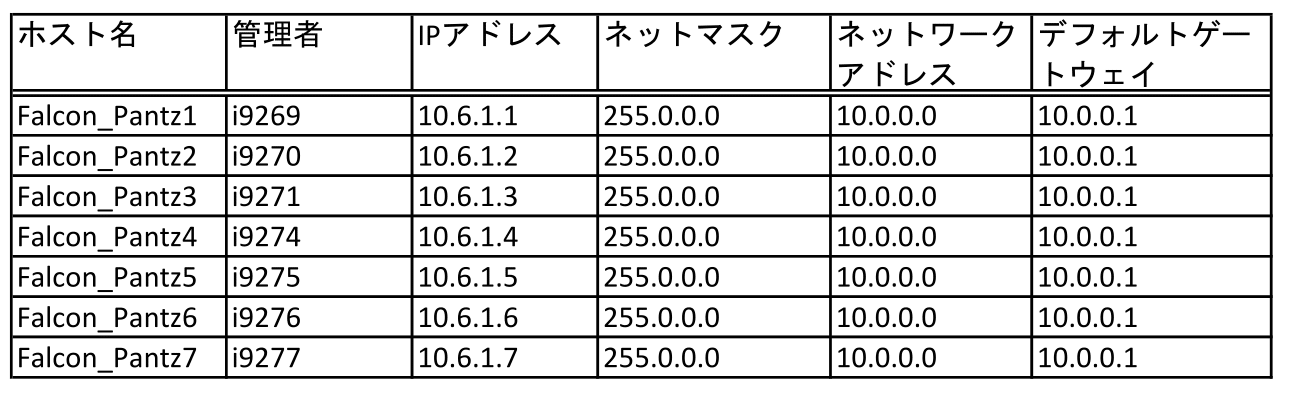
\includegraphics[width=18cm]{3_1.png} \\ \\
                \end{center}
                ホスト名はFalcon\_pantzでIPアドレスは10.6.1.n(nは班のメンバーの番号)を用いた。ネットマスクは上位8bitで、ネットワークアドレスは10.0.0.0を用いた。デフォルトゲートウェイはルーター(c2611r)へつなぐのでそのipアドレス10.0.0.1を用いた。
            \subsection*{3.1.2 課題3-2}
                図24にネットワーク図を示す。図24のように表すネットワークを構築する。また、図25, 26, 27に編集後の設定ファイル、rc.conf, networks, hostsファイルを示す。
                \begin{figure}[H]
                    \begin{center}
                        \begin{screen}
                            \begin{verbatim}
#
# -- sysinstall generated deltas -- # Mon Apr 25 01:01:02 2016
# Created: Mon Apr 25 01:01:02 2016  
# Enable network daemons for user convenience.
# Please make all changes to this file, not to /etc/defaults/rc.conf.
# This file now contains just the overrides from /etc/defaults/rc.conf.
#

check_quotas="NO"
defaultrouter="10.0.0.1"
hostname="falcon_pantz2.exp.info.nara-k.ac.jp"
ifconfig_xl0="inet 10.6.1.2  netmask 255.0.0.0"
sendmail_enable="NONE"
ntpd_enable="YES"
ntpd_flags="-p /var/run/ntpd.pid -f /var/db/ntpd.drift"
inetd_enable="YES"
sshd_enable="YES"

nfs_client_enable="YES"
linux_enable="YES"
sendmail_enable="NONE"

keymap="jp.106x"
moused_enable="YES"
hald_enable="YES"
dbus_enable="YES"
polkitd_enable="YES"
canna_enable="YES"
canna_flags="-u bin -inet"
                            \end{verbatim}
                        \end{screen}
                        \caption{rc.conf}
                        \label{26}
                    \end{center}
                \end{figure}
                \begin{figure}[H]
                    \begin{center}
                        \begin{screen}
                            \begin{verbatim}
#
# $FreeBSD: src/etc/networks, v 01.01.02 2016/04/25 20:12:24 kensmith Exp $
#   @(#)networks    5.1 (Berkeley) 6/30/90
#
# Your Local Networks Database
#
pantznet    10.0.0.0
                            \end{verbatim}
                        \end{screen}
                        \caption{networks}
                        \label{27}
                    \end{center}
                \end{figure}
                \begin{figure}[H]
                    \begin{center}
                        \begin{screen}
                            \begin{verbatim}
#
# $FreeBSD: src/etc/hosts, v 01.01.02 2016/04/25 20:12:24 kensmith Exp $
#       @(#)hosts       5.1 (Berkeley) 6/30/90
#       /etc/hosts (Host Database)
#
# This file should contain the addresses and aliases for local hosts that
# share this file.  Replace 'my.domain' below with the domainname of your
# machine.
#
# In the presence of the domain name service or NIS, this file may
# not be consulted at all; see /etc/nsswitch.conf for the resolution order.
#

#
# IP_address    FQDN  Hostname  [alias1]  [alias2 ...]
#
127.0.0.1   localhost.exp.info.nara-k.ac.jp localhost   # IPv4 loopback
::1     localhost.exp.info.nara-k.ac.jp localhost   # IPv6 loopback

#
#       PC
#
10.6.1.1    falcon_pantz1.exp.info.nara-k.ac.jp falcon_pantz1
10.6.1.2    falcon_pantz2.exp.info.nara-k.ac.jp falcon_pantz2
10.6.1.3    falcon_pantz3.exp.info.nara-k.ac.jp falcon_pantz3
10.6.1.4    falcon_pantz4.exp.info.nara-k.ac.jp falcon_pantz4
10.6.1.5    falcon_pantz5.exp.info.nara-k.ac.jp falcon_pantz5
10.6.1.6    falcon_pantz6.exp.info.nara-k.ac.jp falcon_pantz6
10.6.1.7    falcon_pantz7.exp.info.nara-k.ac.jp falcon_pantz7

#
#       Network Printer
#
172.16.255.1    colorps.exp.info.nara-k.ac.jp colorps       # Color Printer

#
#       Server / Gateway
#
10.255.255.250  pegasus.exp.info.nara-k.ac.jp pegasus       # FreeBSD
10.255.255.251  sleipnir.exp.info.nara-k.ac.jp sleipnir     # FreeBSD
10.255.255.252  phoenix.exp.info.nara-k.ac.jp phoenix       # FreeBSD
10.255.255.253  unicorn.exp.info.nara-k.ac.jp unicorn       # FreeBSD

10.0.0.1    c2611r.exp.info.nara-k.ac.jp c2611r gateway # CISCO 2611R
                            \end{verbatim}
                        \end{screen}
                        \caption{hosts}
                        \label{28}
                    \end{center}
                \end{figure}
                rc.confは図26に示すようにIPアドレス、ホスト名、サブネットマスクを設定した。networksでは図27に示すようにPantznetという名前とネットワークアドレスを設定した。hostsでは図28に示すようにfalcon\_pantzN(Nは班のメンバーの番号)を設定した。これにより、ネットワークの構築を完成させることができた。
            \subsection*{3.1.3 課題3-3}
                ログインホストからlocalhostに対して、以下に示す2通りの条件下におけるpingコマンドの実行結果を示す。
                条件(1) LANケーブルを接続していない状態
                条件(2) LANケーブルを接続している状態
                図29、図30に条件(1)と条件(2)のlocalhostへのpingコマンドを示す。
                \begin{figure}[H]
                    \begin{center}
                        \begin{screen}
                            \begin{verbatim}
i9270@falcon_pantz2<~>$ ping -c 5 localhost
PING localhost (127.0.0.1): 56 data bytes
64 bytes from 127.0.0.1: icmp_seq=0 ttl=64 time=0.012 ms
64 bytes from 127.0.0.1: icmp_seq=1 ttl=64 time=0.004 ms
64 bytes from 127.0.0.1: icmp_seq=2 ttl=64 time=0.007 ms
64 bytes from 127.0.0.1: icmp_seq=3 ttl=64 time=0.004 ms
64 bytes from 127.0.0.1: icmp_seq=4 ttl=64 time=0.006 ms

--- localhost ping statistics ---
5 packets transmitted, 5 packets received, 0.0% packet loss
round-trip min/avg/max/stddev = 0.004/0.007/0.012/0.003 ms
                            \end{verbatim}
                        \end{screen}
                        \caption{localhostへのpingコマンド(条件(1))}
                        \label{29}
                    \end{center}
                \end{figure}
                \begin{figure}[H]
                    \begin{center}
                        \begin{screen}
                            \begin{verbatim}
i9270@falcon_pantz2<~>$ ping -c 5 localhost
PING localhost (127.0.0.1): 56 data bytes
64 bytes from 127.0.0.1: icmp_seq=0 ttl=64 time=0.012 ms
64 bytes from 127.0.0.1: icmp_seq=1 ttl=64 time=0.004 ms
64 bytes from 127.0.0.1: icmp_seq=2 ttl=64 time=0.007 ms
64 bytes from 127.0.0.1: icmp_seq=3 ttl=64 time=0.004 ms
64 bytes from 127.0.0.1: icmp_seq=4 ttl=64 time=0.006 ms

--- localhost ping statistics ---
5 packets transmitted, 5 packets received, 0.0% packet loss
round-trip min/avg/max/stddev = 0.004/0.007/0.012/0.003 ms
                            \end{verbatim}
                        \end{screen}
                        \caption{localhostへのpingコマンド(条件(2))}
                        \label{30}
                    \end{center}
                \end{figure}
                図29、図30から、localhostへのpingはLANケーブルをつないでいてもつないでいなくても速度は変わらないことが分かった。
            \subsection*{3.1.4 課題3-4}
                ログインホストからファイルサーバー(phoenix)に対して、以下に示す3通りの条件下におけるpingコマンドの実行結果を示す。
                条件(1) LANケーブルを接続していない状態
                条件(2) LANケーブルを接続している状態
                条件(3) LANケーブルを接続し、ネットワークインターフェイスx10を無効化している状態
                図31、図32, 図33に条件(1)と条件(2)、条件(3)のphoenixへのpingコマンドを示す。
                \begin{figure}[H]
                    \begin{center}
                        \begin{screen}
                            \begin{verbatim}
i9270@falcon_pantz2<~>$ ping -c 5 phoenix
PING phoenix (10.255.255.252): 56 data bytes

--- phoenix ping statistics ---
5 packets transmitted, 0 packets received, 100.0% packet loss
                            \end{verbatim}
                        \end{screen}
                        \caption{phoenixへのpingコマンド(条件(1))}
                        \label{31}
                    \end{center}
                \end{figure}

                \begin{figure}[H]
                    \begin{center}
                        \begin{screen}
                            \begin{verbatim}
i9270@falcon_pantz2<~>$ ping -c 5 phoenix
PING phoenix.exp.info.nara-k.ac.jp (10.255.255.252): 56 data bytes
64 bytes from 10.255.255.252: icmp_seq=0 ttl=64 time=0.282 ms
64 bytes from 10.255.255.252: icmp_seq=1 ttl=64 time=0.411 ms
64 bytes from 10.255.255.252: icmp_seq=2 ttl=64 time=0.288 ms
64 bytes from 10.255.255.252: icmp_seq=3 ttl=64 time=0.353 ms
64 bytes from 10.255.255.252: icmp_seq=4 ttl=64 time=0.400 ms

--- phoenix.exp.info.nara-k.ac.jp ping statistics ---
5 packets transmitted, 5 packets received, 0.0% packet loss
round-trip min/avg/max/stddev = 0.282/0.3468/0.411/0.060 ms
                            \end{verbatim}
                        \end{screen}
                        \caption{phoenixへのpingコマンド(条件(2))}
                        \label{32}
                    \end{center}
                \end{figure}
                \begin{figure}[H]
                    \begin{center}
                        \begin{screen}
                            \begin{verbatim}
i9270@falcon_pantz2<~>$ ping -c 5 phoenix
PING phoenix.exp.info.nara-k.ac.jp (10.255.255.252): 56 data bytes
ping: sendto:Network is down
ping: sendto:Network is down
ping: sendto:Network is down
ping: sendto:Network is down
ping: sendto:Network is down

--- phoenix.exp.info.nara-k.ac.jp ping statistics ---
5 packets transmitted, 0 packets received, 100.0% packet loss
                            \end{verbatim}
                        \end{screen}
                        \caption{phoenixへのpingコマンド(条件(3))}
                        \label{33}
                    \end{center}
                \end{figure}
                図31, 図33より、LANケーブルにつながっていないときとネットワークインターフェイスを無効化しているときはpoenixにはつなぐことはできなかった。図32のLANケーブルがつながっているときのみpoenixにつなぐことができた。
            \subsection*{3.1.5 課題3-5}
                各ホストのMACアドレスを調べ、表2に示す。
            \subsection*{3.1.6 課題3-6}
                実験メンバー全員の端末接続を確認後ログインホストからブロードキャストアドレスに対してpingコマンドの実行結果を図34に示す。
                \begin{figure}[H]
                    \begin{center}
                        \begin{screen}
                            \begin{verbatim}
i9270@falcon_pantz2<~>$ ping -c 1 10.255.255.255
PING 10.255.255.255 (10.255.255.255): 56 data bytes
64 bytes from 10.255.255.255: icmp_seq=0 ttl=64 time=0.154 ms

--- 10.255.255.255 ping statistics ---
1 packets transmitted, 1 packets received, 0.0% packet loss
round-trip min/avg/max/stddev = 0.154/0.154/0.154/0.000 ms
                            \end{verbatim}
                        \end{screen}
                        \caption{ブロードキャストアドレスへのping}
                        \label{34}
                    \end{center}
                \end{figure}
                ブロードキャストアドレスはサブネットマスクが上位8bitでネットワークアドレスが10.0.0.0などで10.255.255.255となる。図34のようにコマンドを打つことによって結果が得られた。
            \subsection*{3.1.7 課題3-7}
                情報工学科のWebサーバー(www.info.nara-k.ac.jp)に対して、pingコマンドの実行結果を図35に示す。
                \begin{figure}[H]
                    \begin{center}
                        \begin{screen}
                            \begin{verbatim}
i9270@falcon_pantz2<~>$ ping -c 1 www.info.nara-k.ac.jp
PING www.info.nara-k.ac.jp (202.24.246.1): 56 data bytes
64 bytes from 202.24.246.1: icmp_seq=0 ttl=63 time=1.733 ms

--- 10.255.255.255 ping statistics ---
1 packets transmitted, 1 packets received, 0.0% packet loss
round-trip min/avg/max/stddev = 1.733/1.733/1.733/0.000 ms
                            \end{verbatim}
                        \end{screen}
                        \caption{www.info.nara-k.ac.jpへのping}
                        \label{34}
                    \end{center}
                \end{figure}
                図35より、外部のネットワークであるため、帰ってくるまでの時間が1.733msと遅いことが分かった。
            \subsection*{3.1.8 課題3-8}
                ログインホストからファイルサーバーに対して、以下に示す2とおりの条件下におけるpingコマンドの実行結果を図36, 37に示す。
                条件(1) ファイルサーバー(phoenix)のACアドレスがARPテーブルに登録されている状態
                条件(2) ファイルサーバー(phoenix)のACアドレスがARPテーブルに登録されていない状態
                \begin{figure}[H]
                    \begin{center}
                        \begin{screen}
                            \begin{verbatim}
i9270@falcon_pantz2<~>$ ping -c 1 phoenix
PING phoenix.exp.info.nara-k.ac.jp (10.255.255.252): 56 data bytes
64 bytes from 10.255.255.252: icmp_seq=0 ttl=64 time=0.282 ms

--- phoenix.exp.info.nara-k.ac.jp ping statistics ---
1 packets transmitted, 1 packets received, 0.0% packet loss
round-trip min/avg/max/stddev = 0.282/0.282/0.282/0.000 ms
                            \end{verbatim}
                        \end{screen}
                        \caption{phoenixへのping(条件(1))}
                        \label{36}
                    \end{center}
                \end{figure}
                \begin{figure}[H]
                    \begin{center}
                        \begin{screen}
                            \begin{verbatim}
i9270@falcon_pantz2<~>$ ping -c 1 phoenix
PING phoenix.exp.info.nara-k.ac.jp (10.255.255.252): 56 data bytes
64 bytes from 10.255.255.252: icmp_seq=0 ttl=64 time=0.243 ms

--- phoenix.exp.info.nara-k.ac.jp ping statistics ---
1 packets transmitted, 1 packets received, 0.0% packet loss
round-trip min/avg/max/stddev = 0.243/0.243/0.243/0.000 ms
                            \end{verbatim}
                        \end{screen}
                        \caption{phoenixへのping(条件(2))}
                        \label{37}
                    \end{center}
                \end{figure}
                図36、図37より若干ARPテーブルに登録されている状態のほうが速度が速いことが確認できた。
            \subsection*{3.1.9 課題3-9}
                ログインホストにおけるルーティングテーブルを図38に示す。
                \begin{figure}[H]
                    \begin{center}
                        \begin{screen}
                            \begin{verbatim}
i9270@falcon_pantz2<~>$ netstat -r
Routing tables

Internet:
Destination        Gateway       Flags       Refs       Use     Netif Expire
default            c2611r        UGS            0        10        x10
10.0.0.0           link#1        U              0       178        x10
falcon_pantz2      link#1        UHS            0         5        lo0
localhost          link#3        UH             0         1        lo0

Internet6:
Destination        Gateway            Flags      Netif Expire
localhost.exp.info localhost.exp.info UH          lo0
fe80::%lo0         link#3             U           lo0
fe80::1%lo0        link#3             UHS         lo0
ff01::3::          fe80::1%lo0        U           lo0
ff02::%lo0         fe80::1%lo0        U           lo0
                            \end{verbatim}
                        \end{screen}
                        \caption{ルーティングテーブル}
                        \label{38}
                    \end{center}
                \end{figure}
                図38のようにnetstat -rというコマンドでルーティングテーブルを表示することができた。
            \subsection*{3.1.10 課題3-10}
                tracerouteコマンドを使用して、ログインホストから以下に示すホストまでの通信経路を示す。
                ルーター(c2611r)
                ファイルサーバー(phoenix)
                情報工学科のWebサーバー(www.info.nara-k.ac.jp)
                図39にtracerouteコマンドを使用した結果を示す。
                \begin{figure}[H]
                    \begin{center}
                        \begin{screen}
                            \begin{verbatim}
i9270@falcon_pantz2<~>$ traceroute c2611r
traceroute to c2611r.exp.info.nara-k.ac.jp (10.0.0.1), 64 hops max, 40 byte packets
 1 c2611r (10.0.0.1)  2.034 ms *  1.202 ms

i9270@falcon_pantz2<~>$ traceroute phoenix
traceroute to phoenix.exp.info.nara-k.ac.jp (10.255.255.252), 64 hops max, 40 byte packets
 1 phoenix (10.255.255.252)  0.334 ms  0.302 ms  0.237 ms

i9270@falcon_pantz2<~>$ traceroute www.info.nara-k.ac.jp
traceroute to zeus.info.nara-k.ac.jp (202.24.246.1), 64 hops max, 40 byte packets
 1 c2611r (10.0.0.1)  1.903 ms   1.892 ms  1.001 ms
 2 zeus.info.nara-k.ac.jp (202.24.246.1)  2.454 ms  2.455ms  2.390 ms
                            \end{verbatim}
                        \end{screen}
                        \caption{tracerouteコマンド}
                        \label{39}
                    \end{center}
                \end{figure}
                tracerouteのコマンドの引数にホスト名を入れることでそれぞれのホストへの通信経路を表示することができた。
            \subsection*{3.1.11 課題3-11}
                telnetコマンドを使用してそれぞれのホストにログインし、自分のパスワードを設定する。図40にtelnetコマンドを用いたリモート接続のコマンドを示す。
                \begin{figure}[H]
                    \begin{center}
                        \begin{screen}
                            \begin{verbatim}
i9270@falcon_pantz2<~>$ telnet falcon_pantz1
i9270@falcon_pantz1<~>$ passwd i9270
                            \end{verbatim}
                        \end{screen}
                        \caption{telnetを用いたリモートアクセス}
                        \label{40}
                    \end{center}
                \end{figure}
                図39のようにtelnetコマンドの引数にホスト名をいれて、そのコンピュータにアクセスしpasswdコマンドでパスワードを変更した。図39はfalcon_pantz1だけだが、これをfalconpantz7まですべてに実行した。
            \subsection*{3.1.12 課題3-12}
                rloginコマンドを使用してそれぞれのホストにパスワードチェックを省略してログインできるようにユーザーレベルによる設定を行う。図41と図42にログイン時のパスワードのチェックを省略させるコマンドとloginを用いたログインを示す。
                \begin{figure}[H]
                    \begin{center}
                        \begin{screen}
                            \begin{verbatim}
i9270@falcon_pantz1<~>$ echo falcon_pantz2 > .rhosts
                            \end{verbatim}
                        \end{screen}
                        \caption{パスワードチェックを省略する作業}
                        \label{41}
                    \end{center}
                \end{figure}
                \begin{figure}[H]
                    \begin{center}
                        \begin{screen}
                            \begin{verbatim}
i9270@falcon_pantz2<~>$ rlogin falcon_pantz1
i9270@falcon_pantz1<~>$ 
                            \end{verbatim}
                        \end{screen}
                        \caption{rloginコマンド}
                        \label{42}
                    \end{center}
                \end{figure}
                図41、42のように.rhostsファイルの中にホスト名を入れることによってそのホストからのログイン時にパスワードが不要になるということが分かった。

        \section*{4.1 課題4 ネットワークの性能とネットワーク機器の特徴}
            \subsection*{4.1.1  課題4-1}
            \subsection*{4.1.1  課題4-2}
            \subsection*{4.1.1  課題4-3}
            \subsection*{4.1.4  課題4-4}
            \subsection*{4.1.5  初級問題}
            \subsection*{4.1.6  中級問題}

    \chapter*{第3章 実験結果の考察および検討}
            \section*{3.1 課題考察}
                \subsection*{3.1.1 TCPとUDPの通信方式}
                \subsection*{3.1.1 ルーティングプロトコル}
                    ルーティングプロトコルは大きく分けて2つに分類できる。1つはRIP, OSPF, EIGRPなどのIGPとBGPなどのEGPである。以下にそれぞれの特徴を示す.
                    \begin{itemize}
                    \item RIP: ディスタンスベクタ型
                    \item OSPF: 
                    \item EIGRP: 
                    \item BGP: 
                \end{itemize}
                \subsection*{3.1.1 DNS}

                \subsection*{3.1.1 QoS}

            \section*{3.2 自由考察}
                \subsection*{3.1.1 RSA}
                    公開鍵暗号方式の一つである。大きな素数p, qを生成し、n=pqとする。(p - 1)(q - 1)とお互いにそな整数k1を取ってくる。k1k2=1mod(p - 1)(q - 1)なるk2を取ってくる。公開鍵はnとk1, 秘密鍵はk2となる。ここで、メッセージを送る場合は、送りたいメッセージをmとし、公開鍵を用いてm^k_1modnを計算する。逆にメッセージを受け取る側は秘密鍵を用いてC^k_2modnを計算すると元々のメッセージを求められる。これは、暗号文と公開鍵が分かっていても、時間がかかりすぎて、秘密鍵mが求められないという理由よりこの暗号は解けないというものである。つまり、このままコンピュータの性能が上がっていけば、いつかは、解読できる日かくるかもしれないということである。ある一つの文献では、2100年ごろであると言われています。(Qiita ssh暗号化はRSAでいいのか より)
                \subsection*{3.1.1 衛星によるインターネット環境}
                    現在、世界中の人間の中で貧困などの理由より57\%はインターネットを利用することができないと言われる。そこで、世界中の人があらゆる場所でインターネットを使えるようにするためのプロジェクトをGoogleなど様々な企業、やまたは国が進めている。中でもFacebookのInternet.orgというプロジェクトでは、今年(2016年)に人工衛星を打ち上げアフリカを中心に安価でインターネットを利用できるようになるのだそう。世界中のひとがインターネットを利用できるようになるまではそれほど、時間はかからないようである。


    \chapter*{第4章 参考文献および参考URL}

    \chapter*{第5章 実験における意見や感想}
        \section*{5.1 実験指導書に対する意見や感想}
            指導書にコマンドなどの使い方を書くのではなく、インターネットで調べさせる方が、実際に業務で何かしたいと思った時にそれをできるようになる能力が付くと思う。指導書内に記述欄は必要ないので、コマンドの実行結果を保存するシステムが欲しい。(例えば、USBにコマンドの実行結果を移すなど。) 
        \section*{5.2 実験課題に対する意見や感想}
            telnet, rloginは今はあんまり使われないと思うので、telnet, rloginの課題は無くすべきである。その代わりに、一番最初にsshの設定を行い、クライアントPCからアクセスして今回の課題をするべきだったと思う。LANケーブルを作成する課題はいらない。実際にルーターにもアクセスして設定させて欲しかった。
        \section*{5.3 e-Learningシステムに対する意見や感想}
            非常に楽である。学校内のe-learningをなくして、全部今回のmoodleにしてほしい。
        \section*{5.4 コンピュータネットワークに関する実験全体の感想}
            生徒たちがどれだけ、UNIXについての知識を持っているかというのを考慮していない、実験内容であると思う。生徒たちにとってwindowsは使うことは多々あったのである程度わかるが、UNIXについては全く無知の状態から入るため、先生たちの説明すら全く理解できないと思う。今回の実験メンバーの場合、完璧に理解していたのは僕と黒田君ぐらいではないでしょうか。。OSは会社でよく使われるRedHat系のOSで実験を行う方が将来役立つと思う。
        \section*{5.5 この実験を通して私が得た、発見した、気付いたこと}
            ネットワークの授業でPackettracerを用いて学んだことをが役に立った。少し、UNIXのコマンドの知識が増えた。ネットワークの知識については、staticでルーティングをすることができるようには多分なったと思う。
        \section*{5.6 その他}
            全体を通して、充実した実験だったと思う。4年になっていきなりこの実験はきつかったので、3年の実験にもうちょっと軽めでネットワーク、UNIXの実験があれば、もう少し楽に楽しく実験を行うことができたと思う。この実験でUNIX嫌いになった人が多いんじゃないのかなあ。
    \chapter*{第6章 テキストの訂正}

\end{document}
